% Template for Elsevier CRC journal article
% version 1.2 dated 09 May 2011

% This file (c) 2009-2011 Elsevier Ltd.  Modifications may be freely made,
% provided the edited file is saved under a different name

% This file contains modifications for Procedia Computer Science

%-----------------------------------------------------------------------------------

\documentclass[3p,times,procedia]{elsarticle}
\flushbottom

\usepackage{ecrc}
\usepackage[bookmarks=false]{hyperref}
\hypersetup{
  colorlinks,
  linkcolor=blue,
  citecolor=blue,
  urlcolor=blue
}
\usepackage{graphicx}
\usepackage{amssymb}
\usepackage{booktabs}

\volume{00}
\firstpage{1}
\journalname{Procedia Computer Science}
\runauth{Gheorghe et al.}
\jid{procs}

\begin{document}
\begin{frontmatter}

\dochead{30th International Conference on Knowledge-Based and Intelligent Information \& Engineering Systems (KES 2026)}

\title{Robust Agentic AI for Public Administration: A Multi-Agent Architecture and Controlled Fault Injection Evaluation}

\author[a,b]{Radu-Mihai Gheorghe}
\author[b]{Petru-Liviu Bouruc}
\author[b]{Ciprian Paduraru}
\author[b,c]{Alin Stefanescu}

\address[a]{UiPath, Romania}
\address[b]{University of Bucharest, Romania}
\address[c]{Institute for Logic and Data Science, Romania}

\begin{abstract}
\textbf{BACKGROUND:} The digital transformation of public administration requires intelligent systems that guide citizens through complex regulatory workflows while remaining reliable under the integration faults that arise in production environments. Agentic AI systems, in which large language models coordinate specialised agents across multi-step workflows, offer a promising path toward unified interfaces for fragmented public services, yet their robustness under realistic service failures remains poorly understood. \textbf{OBJECTIVES:} This paper presents a multi-agent architecture for public administration services and evaluates its robustness under controlled fault injection conditions, with the goal of quantifying how many integration failures propagate silently to citizens and assessing the financial feasibility of institutional adoption. \textbf{METHODS:} The architecture is instantiated for Romanian tax and fiscal administration using the open-source UiPath Python SDK and LangGraph. It includes an intent-routing orchestration layer, five domain-specific agents covering freelancer tax contributions under the PFA (\textit{persoan\u{a} fizic\u{a} autorizat\u{a}}, in Romanian; self-employed status) regime, property sale taxation, rental income obligations, fiscal certificate issuance, and electronic invoicing through RO e-Factura, together with a shared services layer for retrieval-augmented generation over the Romanian Tax Code, deterministic tax computation, document processing, and payment handling. Robustness is evaluated through a controlled fault injection framework that instruments 19 external service boundary operations---each receiving at most one independently drawn fault---with four chaos operators: timeout, delay, partial response, and corruption, applied at configurable rates with a seeded random number generator for reproducibility. \textbf{RESULTS:} Experiments over 100 individual boundary calls reveal a structural silent pass-through rate of approximately 63\%: faults that do not affect the downstream branching predicate remain undetected, with the LLM producing plausible citizen-facing responses despite null or corrupted service data. This rate is determined by the operator mix and response schema structure, not by the injection rate, and remains stable across all tested values of $\eta$. LLM inference costs are estimated at approximately \$0.05 per session, scaling to about \$5{,}060 per month for a large agency handling 5{,}000 daily interactions. \textbf{CONCLUSION:} The 63\% silent pass-through rate motivates output-level contract verification as a necessary complement to agentic systems deployed in regulated public services. The implementation and evaluation artefacts are released publicly to support reproducibility and further research.
\end{abstract}
\begin{keyword}
multi-agent systems ; agentic AI ; robustness of agentic AI systems ; fault injection ; chaos engineering ; public administration ; tax automation ; UiPath SDK ; LangGraph
\end{keyword}

\end{frontmatter}

\section{Introduction}
\label{sec:introduction}

The digital transformation of public administration has become a strategic priority across Europe. In Romania, recent initiatives include Romania's National Agency for Fiscal Administration (ANAF) \textit{Spa\c{t}iul Privat Virtual} (SPV; Virtual Private Space, in Romanian) portal for tax declarations, Ghiseul.ro, the national electronic payment platform, and RO e-Factura, the national electronic invoicing system. Although these platforms support important administrative functions, they also impose a substantial burden on citizens and businesses. Users must navigate several interfaces, interpret changing tax regulations, and coordinate across disconnected services to complete routine fiscal tasks. Agentic AI systems, in which large language models (LLMs) coordinate specialised agents, interact with external services, and maintain context across multi-step workflows, offer a plausible way to provide unified conversational access to such fragmented processes \cite{Pan2025, WEF2025}.

\textcolor{red}{Two compatible objectives were taken into consideration when creating this architecture, one for each group it serves. For Romanian taxpayers, individuals and small businesses, the objective is unified conversational access that hides the procedural fragmentation across SPV, Ghiseul.ro, and RO e-Factura behind a single interface, so that routine fiscal tasks no longer require navigating several portals in isolation. For ANAF, which would host such an assistant on top of those portals, the complementary objective is having a unified system with sufficient reliability that it continues to behave coherently when its dependent services are slow, partially available, or return malformed data, since incoherent administrative responses in this domain would undermine the credibility of regulated public services. The remainder of the paper addresses these two objectives in turn: the multi-agent architecture targets the first, and the controlled fault injection evaluation targets the second.}

Deploying such a system in practice requires more than an LLM orchestration library. A bare LangChain or LangGraph implementation still leaves several engineering concerns unresolved, including model access, retrieval infrastructure, retry logic for unreliable integrations, human escalation, and document storage with access control. These concerns become especially important in public administration, where workflows often span multiple systems and where some government portals still depend on browser-based interaction rather than public APIs. In such settings, a practical implementation substrate must support both agent orchestration and operational integration.

The present prototype uses the open-source UiPath Python SDK \cite{UiPathSDK2025} together with LangGraph \cite{LangGraph2025}. This choice is motivated by integration requirements rather than platform preference alone. The SDK supports native LangGraph state machines while also providing orchestration, persistence, monitoring, storage, human-in-the-loop escalation, and retrieval services within the same execution environment. The \texttt{UiPathChat} interface exposes LLM access through the platform gateway, while \texttt{ContextGroundingRetriever} supports retrieval-augmented generation over indexed knowledge bases. The same environment also supports queue-based execution, task creation for human review, and storage buckets for document handling. This reduces the need to assemble and maintain a separate stack for model serving, vector search, workflow state, and operational controls. Within a single execution trace, an agent can classify user intent, retrieve relevant fiscal guidance, compute tax obligations through deterministic services, and coordinate interactions with systems such as SPV and Ghiseul.ro.

However, a workable implementation substrate does not by itself address robustness. In public administration, users expect stable behaviour even when a dependent system is slow, partially unavailable, or returns malformed data. These are ordinary integration failures in production environments, but they are not always exercised explicitly during development. An agent that reacts only to a service-reported success flag may still generate a plausible response when the underlying payload is incomplete or corrupted. This creates a particularly problematic failure mode in regulated settings: the system appears coherent at the interface level while silently propagating invalid state. Analysing this behaviour requires controlled perturbation at the system boundaries, in the spirit of chaos engineering for service-based software \cite{Basiri2016}.
This paper makes three contributions:
\vspace{-2mm}
\begin{enumerate}
    \item A multi-agent architecture for public administration is introduced, in which an Entry Agent performs intent detection and routes requests to one of five domain-specific agents: PFA/Freelancer, Property Sale, Rental Income, Certificate, and E-Factura. These agents share services for document intake, retrieval over the Romanian Tax Code, deterministic tax computation, and payment processing through national platforms such as SPV, Ghiseul.ro, and RO e-Factura.
    \item A fault injection framework is defined for 19 external service boundary operations using four chaos operators: timeout, delay, partial response, and corruption. The framework supports configurable injection rates and deterministic replay through a seeded random number generator. Across injection rates from 0\% to 100\%, the experiments show that approximately 63\% of injected faults propagate silently when the affected fields do not alter the downstream branching predicate.
    \item An openly available implementation of the architecture and evaluation setup is provided to support reproducibility and further research on robust agentic systems for regulated public services.
\end{enumerate}

The architecture follows a hierarchical supervisor topology \cite{AutoGen2023} implemented with LangGraph's \texttt{StateGraph} and conditional routing. Its orchestration and shared services layers are designed to be reusable across public service domains, while the present instantiation focuses on Romanian tax and fiscal administration: freelancer taxation under the PFA (\textit{persoan\u{a} fizic\u{a} autorizat\u{a}}, in Romanian; self-employed status) regime and \textit{Declara\c{t}ia Unic\u{a}} (D212; Single Tax Return, in Romanian), property transactions, rental income, fiscal certification, and electronic invoicing. These workflows provide a representative example of the procedural fragmentation and regulatory complexity that public-facing intelligent information systems must address.

The central empirical result is structural rather than incidental: many faults remain invisible to the agent when they do not affect the predicate used for control flow. This motivates output-level validation as a necessary complement to agentic systems deployed in regulated public services.


\section{Related Work}
\label{sec:related}

\textit{Agentic AI for digital government and tax services.}
The use of NLP and AI in public administration has evolved from document classification and information extraction toward conversational systems that support multi-step administrative tasks. Jiang et al.~\cite{Jiang2023} identify automation, extension, and transformation as the main contribution patterns across 1{,}032 NLP studies in government contexts. Madan and Ashok~\cite{Madan2022} review barriers to AI adoption in public-sector organisations and emphasise transparency, accountability, and institutional readiness. In tax administration, Nay et al.~\cite{Nay2024} show that GPT-4 combined with retrieval over legal materials can achieve competitive performance on tax-law question answering. At the institutional level, Schmitz et al.~\cite{Schmitz2025} identify governance requirements that should be satisfied before agentic AI systems are adopted in public-sector practice. The present work extends this line of research from advisory question answering to a multi-agent service architecture that supports several operational tax workflows in a concrete national setting.

\textit{Multi-agent architectures and retrieval-augmented generation.}
Wang et al.~\cite{Wang2024survey} describe LLM-based autonomous agents through a common decomposition into profile, memory, planning, and action modules. AutoGen \cite{AutoGen2023} and LangGraph \cite{LangGraph2025} represent two influential implementation styles: the former emphasises conversational multi-agent interaction, whereas the latter provides a typed state-machine model suited to explicit workflow control and long-running execution. The architecture presented here adopts LangGraph's hierarchical supervisor pattern with intent-gated routing. For knowledge grounding, Gao et al.~\cite{Gao2024} provide a broad survey of retrieval-augmented generation, while Pipitone and Houir Alami~\cite{Pipitone2024} examine retrieval quality in legal-domain RAG. Their findings are directly relevant to tax and regulatory assistance, where retrieval precision strongly affects answer quality and traceability.

\textit{Robustness, fault injection, and reliability of LLM agents.}
AgentBench \cite{Liu2024AgentBench} evaluates LLMs as agents across several environments and highlights long-horizon reasoning and instruction following as recurring weaknesses. Rabanser et al.~\cite{Rabanser2026} propose a set of reliability metrics spanning consistency, robustness, and predictability, and show that stronger capability does not automatically yield stronger reliability. Shah et al.~\cite{Shah2026} study faults in open-source agentic repositories and identify failures at the boundary between probabilistic model outputs and deterministic program logic as a dominant class. This is the same interface targeted in the present evaluation. Owotogbe~\cite{Owotogbe2025} applies chaos engineering ideas to LLM-based multi-agent systems through hallucination and communication faults, and Gupta~\cite{Gupta2026} extends this direction with ReliabilityBench, which includes timeout, partial-response, and schema-drift conditions. The contribution here differs in three respects: it studies a regulated public-service setting, it uses a decorator-based injection mechanism that remains separate from agent logic, and it connects the observed silent failure rate to the structure of the response schema and branching predicate.

At the European policy and implementation level, Tangi et al.~\cite{Tangi2026JRC} discuss future directions for advancing AI adoption in EU public administrations, with emphasis on organisational capacity, regulatory alignment, and high-impact public-sector application domains.

\textit{Research gap.}
The three bodies of literature reviewed above converge on an open problem that none of them addresses in combination. Work on AI for government and tax services has so far focused on advisory question answering and single-agent document processing; no published system integrates the full operational stack---orchestration, domain routing, RAG, deterministic computation, and payment handling---for a concrete national fiscal setting. Work on multi-agent architectures and RAG provides the implementation substrate but does not address what happens when the external services these agents depend on fail. Work on robustness and fault injection targets generic agentic benchmarks or synthetic environments; no existing study applies controlled boundary-level fault injection to a regulated public-service architecture, quantifies the fraction of faults that propagate silently through the agent's control flow, or links that fraction analytically to the structure of the response schema. This paper fills the intersection of these three gaps: it introduces an operational multi-agent architecture for a specific national setting and evaluates it under controlled fault injection in a way that is both practically grounded and analytically interpretable.

\section{Methods}
\label{sec:methods}

The research follows a Design Science Research (DSR) methodology~\cite{Hevner2004}, structured around two phases. In the \emph{design and construction phase}, an artefact---the multi-agent architecture---is built to address a practical problem: the fragmentation of public fiscal services and the absence of a unified, conversational interface grounded in authoritative tax-code content. In the \emph{evaluation phase}, the artefact is subjected to a controlled experiment in which integration faults are injected at external service boundaries under varying rates, with outcomes classified and analysed to characterise system robustness. This combination of artefact construction and controlled experimentation is well suited to applied AI systems research, where the scientific contribution lies both in the design of the system and in measurable properties of its behaviour.

This section describes the multi-agent architecture for public administration, instantiated here for Romanian tax and fiscal services, together with the fault injection framework used to evaluate robustness under simulated service failures. The system is organised into five layers: user interface, orchestration, domain agents, shared services, and infrastructure. A separate fault injection layer instruments mocked external boundaries so that controlled perturbations can be introduced during development and testing without requiring live access to government portals.

\subsection{System architecture}
\label{subsec:architecture}

The architecture follows a hierarchical supervisor pattern implemented as a LangGraph \texttt{StateGraph} with typed state and conditional routing. Figure~\ref{fig:architecture} shows the full organisation of the system across the five layers.

\begin{figure}[t]
\centering
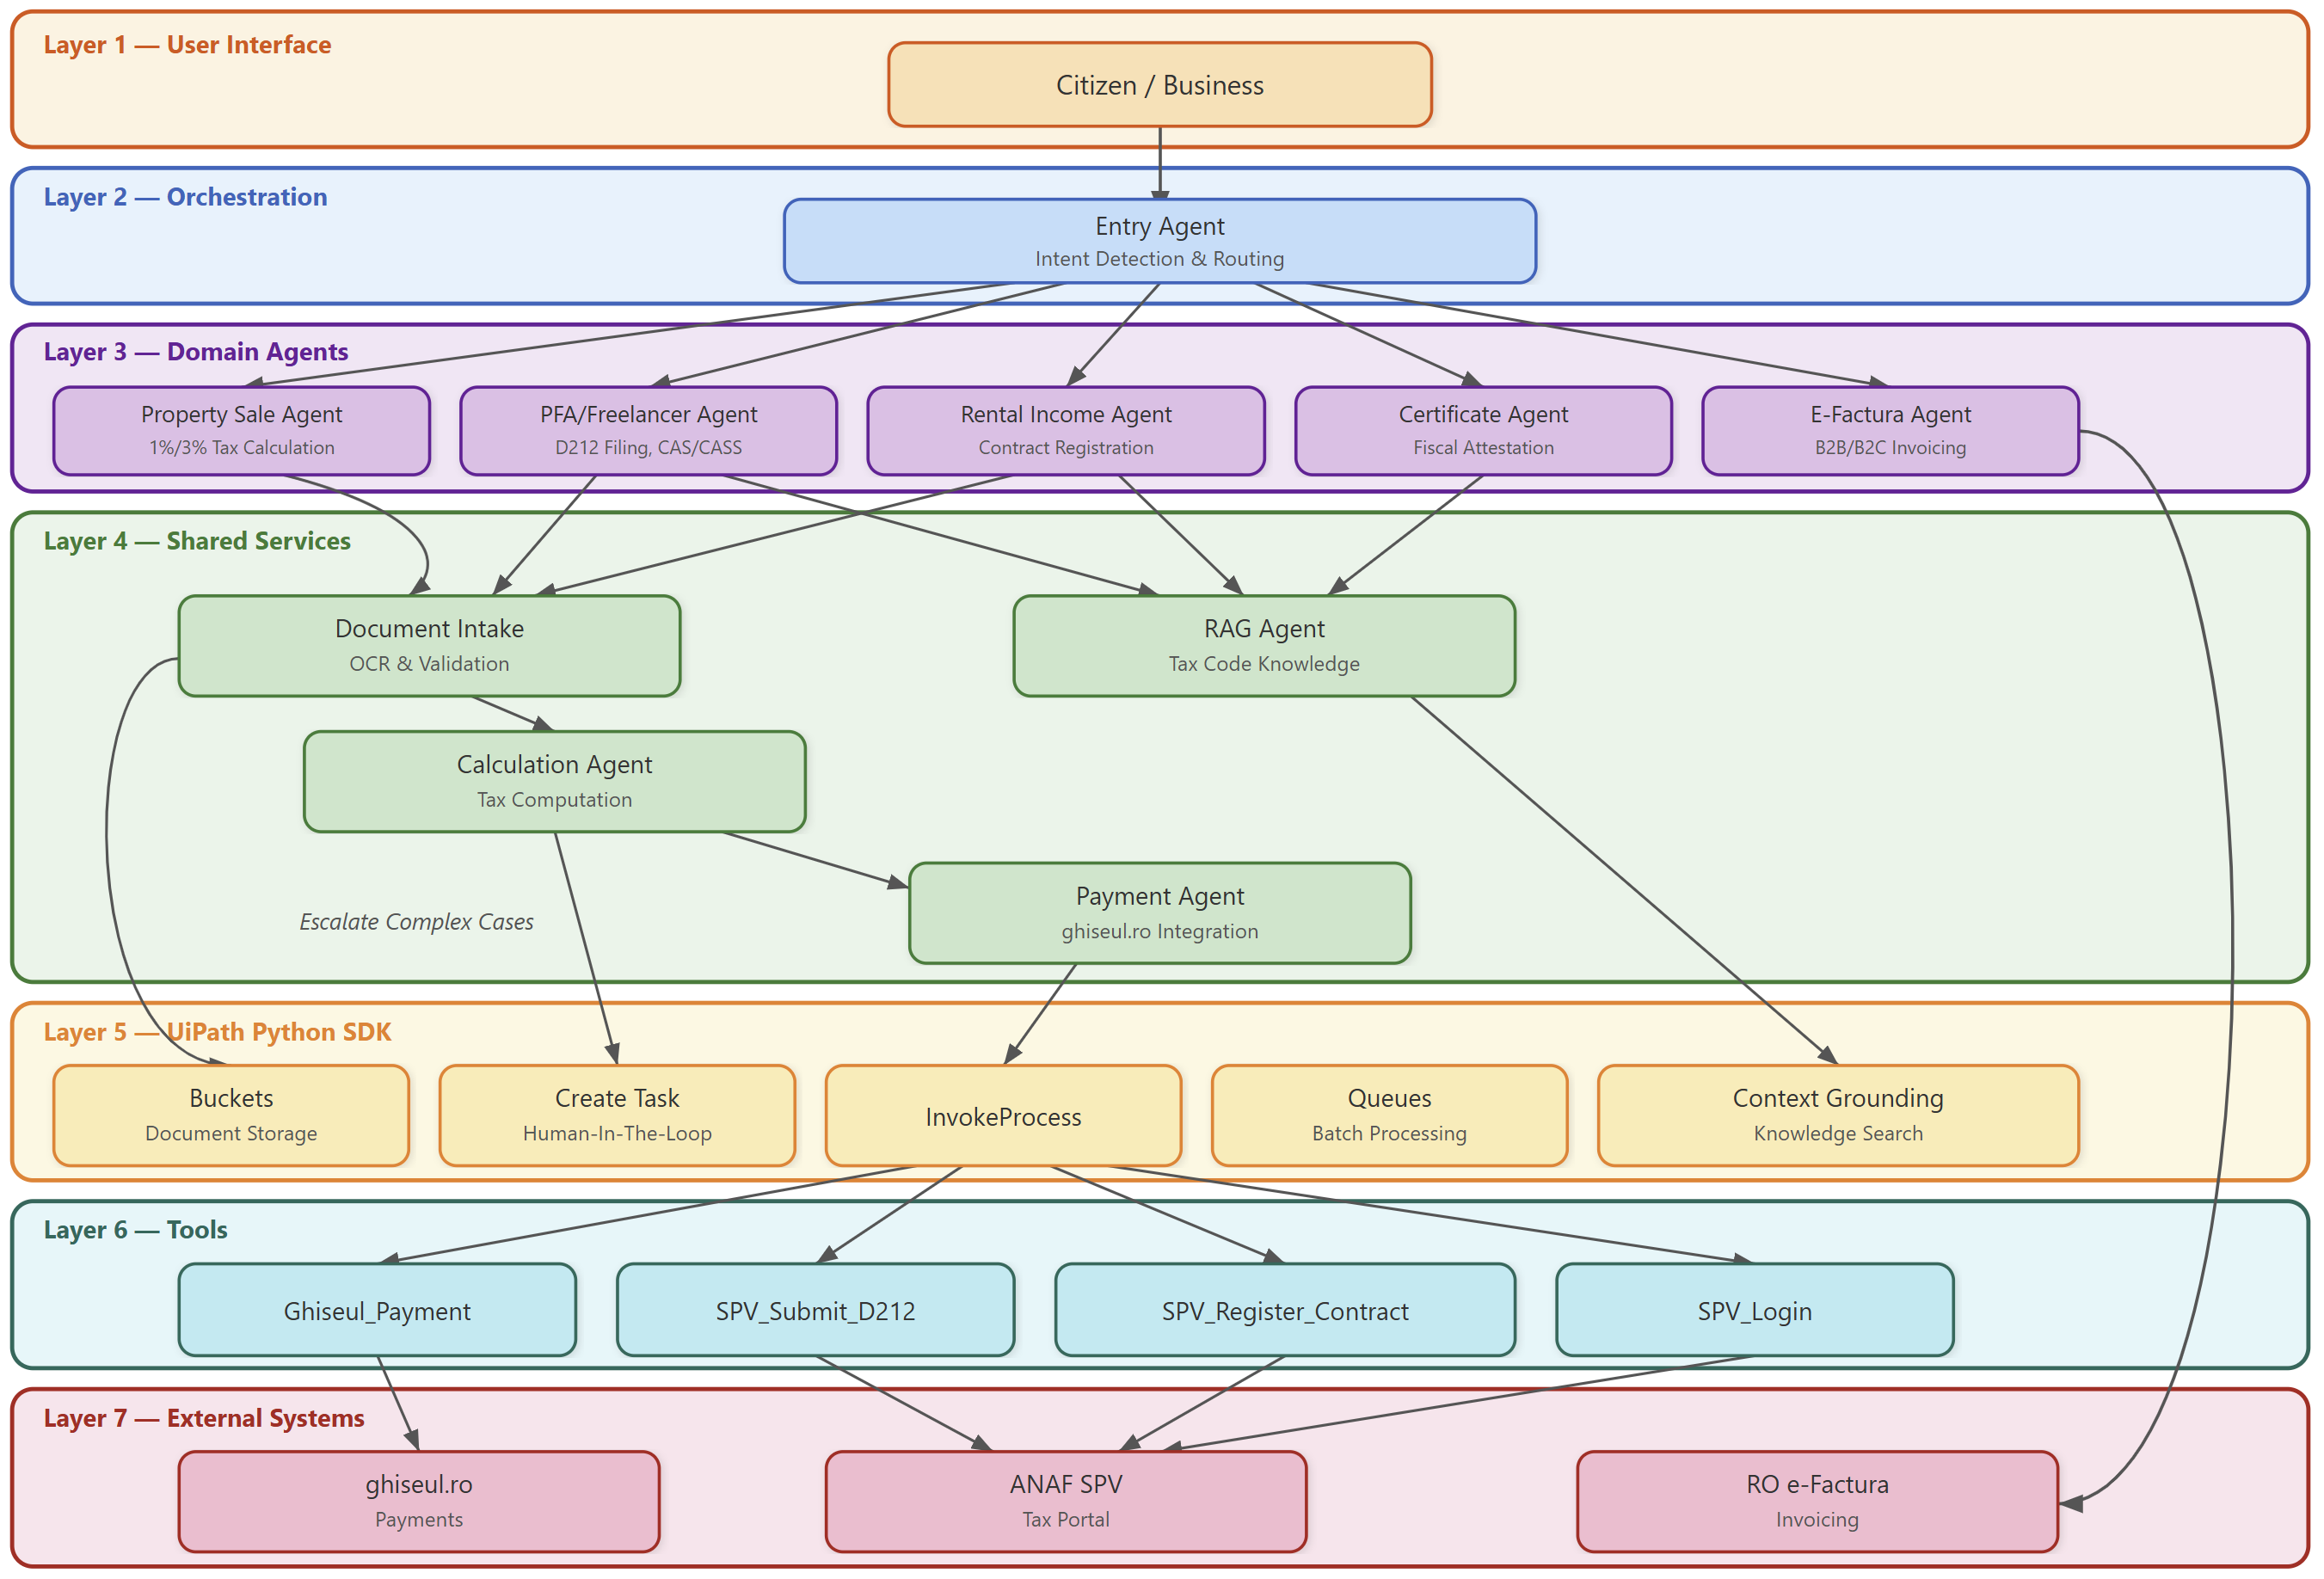
\includegraphics[width=\columnwidth]{updated_architecture_diagram.png}
\caption{Multi-agent architecture for Romanian tax administration. The orchestration layer routes citizen requests through an Entry Agent to domain-specific agents. These agents use shared services for document processing, knowledge retrieval, tax computation, and payments. The infrastructure layer exposes UiPath Orchestrator capabilities and external government systems.}
\label{fig:architecture}
\end{figure}

The system maintains a shared state across graph nodes. This state includes the user query, conversation history, routing fields, intent classification results, workflow status, and a context dictionary for cross-agent data exchange. The graph takes a user query as input and returns the response text together with the detected intent, confidence score, and workflow status.

\subsubsection{Orchestration layer: Entry Agent}
\label{subsubsec:entry}

The Entry Agent is the sole entry point for user interaction and is responsible for intent detection. Given a user query, it invokes an LLM (GPT-4o via the UiPath LLM Gateway) with a system prompt that lists the supported service categories and requests a structured classification. The classifier distinguishes among the supported tax-service workflows, general questions, and unclear requests. It returns the predicted intent, a confidence score, explanatory reasoning, and any domain-specific entities extracted from the user query, such as annual income, property value, ownership duration, monthly rent, or invoice type.

A deterministic mapping translates the classified intent into the corresponding graph node. Routing is then gated by a confidence threshold. If the confidence score falls below the configured threshold, the request is redirected to a clarification node even if an intent has been assigned. This two-stage procedure combines structured LLM classification with deterministic routing and reduces the risk of dispatching ambiguous requests to the wrong domain agent.

\subsubsection{Domain agents layer}
\label{subsubsec:domain}

Five domain-specific agents implement the main tax-service workflows. Each agent receives the shared state, invokes the LLM with a domain-specific prompt, interacts with shared services when necessary, and returns updated state together with response messages.

\paragraph{PFA/Freelancer Agent}
This agent supports filing of \textit{Declara\c{t}ia Unic\u{a}} (D212; Single Tax Return, in Romanian) for self-employed individuals under the PFA regime. It collects income information from user input or extracted entities, delegates social insurance contribution (CAS, pension, 25\%) and health insurance contribution (CASS, 10\%) computation to the Calculation Service, and guides the user through submission via SPV. CAS applies when annual income is at least $12 \times$ the minimum gross salary (48{,}600 RON for 2026) and is computed on the threshold amount. CASS applies when annual income is at least $6 \times$ the minimum gross salary (24{,}300 RON for 2026).

\paragraph{Property Sale Agent}
This agent computes property sale tax according to ownership duration: 3\% for properties held for less than 3 years and 1\% for properties held for 3 years or more. It extracts the property value and holding period, delegates the calculation, and provides payment guidance through Ghiseul.ro.

\paragraph{Rental Income Agent}
This agent supports rental contract registration with ANAF and computes the 10\% flat tax on annual rental income. The workflow includes contract data collection, registration through SPV, and payment support.

\paragraph{Certificate Agent}
This agent assists users in obtaining a \textit{Certificat de atestare fiscal\u{a}} (fiscal attestation certificate, in Romanian). It identifies the required certificate type, checks document requirements, and guides the submission process.

\paragraph{E-Factura Agent}
This agent supports electronic invoicing for both B2B and B2C scenarios. It handles invoice data collection, XML generation consistent with the RO e-Factura standard, submission to the national system, and status monitoring.

All domain agents produce a standardised response field from the final model output, which ensures consistent formatting across workflows.

\subsubsection{Shared services layer}
\label{subsubsec:shared}

Four shared services provide reusable capabilities across all domain agents.

\paragraph{Document Intake Service}
This service processes uploaded documents through OCR and validates extracted data against document-specific schemas. It supports D212 forms, rental contracts, and invoices, and returns structured data together with confidence scores and validation errors. Documents with OCR confidence below 80\% are flagged for manual review.

\paragraph{RAG Service}
This service implements retrieval-augmented generation over dedicated indices containing relevant sections of the Romanian Tax Code and procedural guidance. For a given query, it retrieves the most relevant passages, builds a grounded prompt, and generates an answer conditioned on the retrieved evidence. This supports traceable tax-code interpretation instead of relying solely on parametric model knowledge.

\paragraph{Calculation Service}
This service performs deterministic tax computations using decimal arithmetic to avoid floating-point error in financial calculations. It supports PFA contributions, property sale tax, and rental income tax. All calculations depend on configurable parameters such as minimum salary levels and tax rates, allowing annual regulatory updates without changing code.

\paragraph{Payment Service}
This service integrates with Ghiseul.ro for tax payment processing. It constructs payment requests from the shared context, initiates the payment, and returns transaction details such as a redirect URL for payment completion.

\subsubsection{Infrastructure layer: UiPath platform integration}
\label{subsubsec:infrastructure}

The infrastructure layer connects the agent system to the UiPath Orchestrator platform and, through mocked boundary adapters, to the target government systems. It provides support for robotic process execution, human review tasks, queue-based batch handling, persistent document storage, and retrieval over indexed knowledge sources.

The tools layer exposes mocked functions that mirror the request and response schemas of the corresponding government services, including SPV authentication, D212 submission, rental contract registration, and payment initiation. In production, these functions would be replaced by UiPath robotic processes. The present prototype uses mock implementations to support controlled evaluation while preserving the external interaction structure of the target workflows.

\subsection{Fault injection layer}
\label{subsubsec:faultinjection}

\begin{figure}[t]
\centering
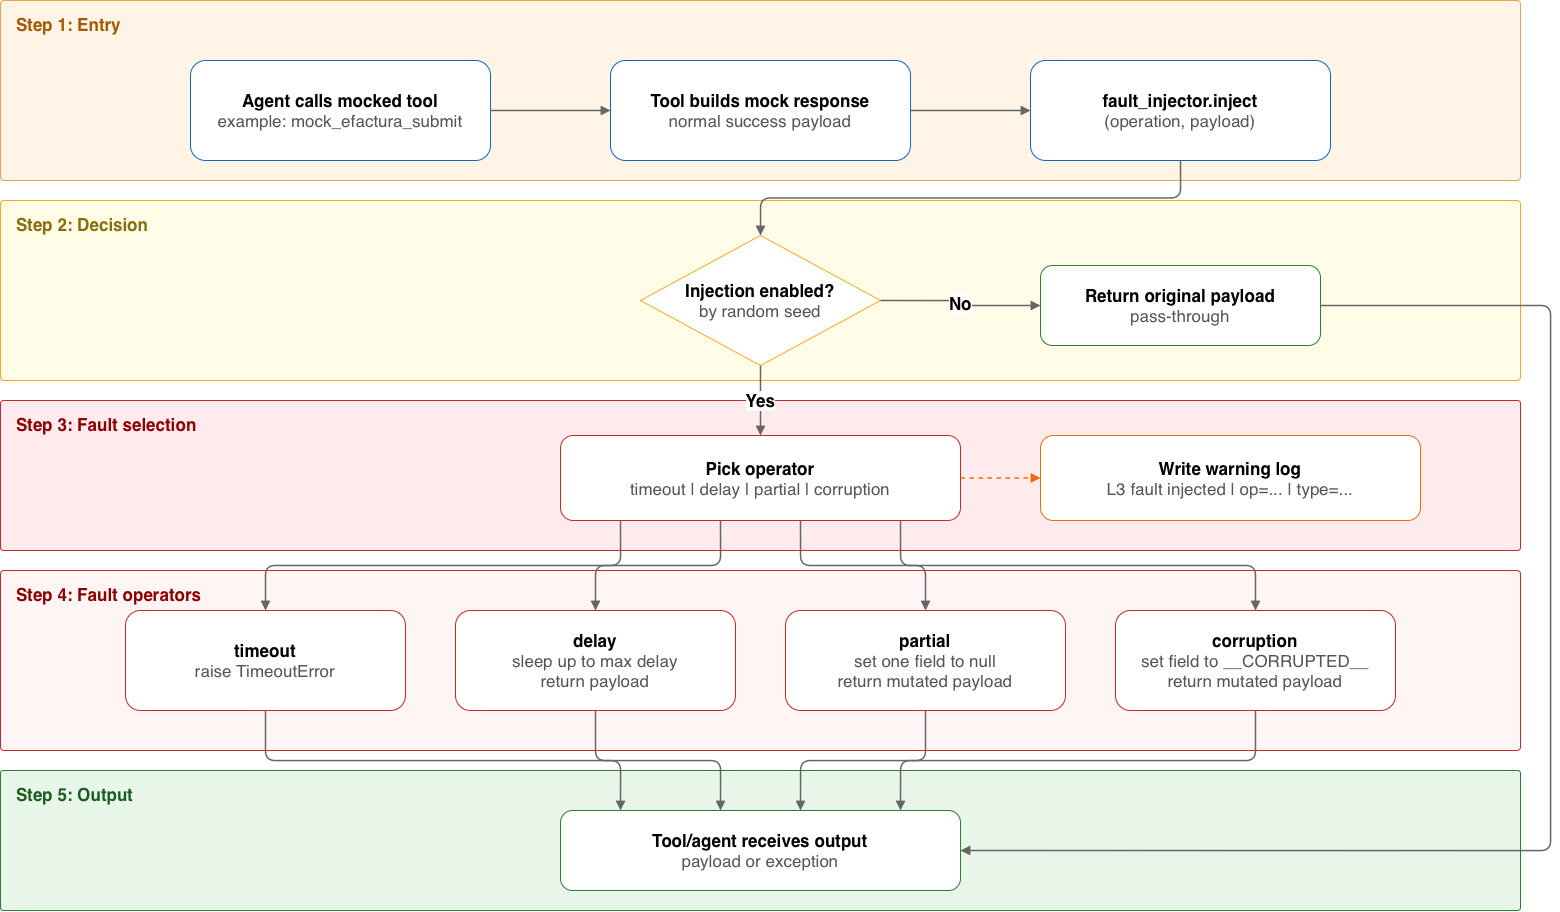
\includegraphics[width=\columnwidth]{PROCS_KES2026_LATEX_Template/l3pngbigtext.drawio.png}
\caption{Fault injection decision flow. When an agent calls a mocked tool, the tool first constructs its nominal response and passes it to the fault injector. A seeded Bernoulli trial determines whether injection occurs. On pass-through, the original payload is returned unchanged. Otherwise, one of four chaos operators is selected uniformly: \emph{timeout} (raises \texttt{TimeoutError}), \emph{delay} (sleeps and returns the payload), \emph{partial} (sets one field to null), or \emph{corruption} (replaces one field with a sentinel value). A warning is written to the fault log before the result is returned to the agent.}
\label{fig:finjarchitecture}
\end{figure}

Production assurance for agentic systems requires robustness not only under nominal operation but also under the integration faults common in deployed environments, including timeouts, partial responses, payload corruption, and communication delays \cite{Basiri2016}. To study these conditions without relying on live government portals, the mocked external boundaries are instrumented with a controlled fault injection framework that applies chaos operators at configurable rates with deterministic reproducibility.

The fault injector is parameterised by a random seed $s$, a per-call injection probability $\eta \in [0,1]$, and a maximum induced latency $\Delta t_{\max}$. Each boundary crossing is treated as an independent trial: at most one fault is injected per call. Specifically, the injector draws a single Bernoulli sample with parameter $\eta$; if the draw fails (probability $1-\eta$) the payload is returned unchanged, and if it succeeds exactly one of four operators is selected uniformly at random and applied to that call alone. Within a multi-step citizen session that crosses $k$ boundaries, up to $k$ faults may accumulate across calls, but they are independent and do not overlap---each call receives one Bernoulli draw and at most one operator. If injection occurs, the selected operator is one of:

\begin{itemize}
\item \textbf{Timeout}: raises a \texttt{TimeoutError} and returns no payload;
\item \textbf{Delay}: sleeps for a duration sampled uniformly from $[1, \Delta t_{\max}]$ ms and then returns the original payload;
\item \textbf{Partial response}: selects one payload field uniformly at random and sets it to \texttt{None}; and
\item \textbf{Corruption}: selects one field and replaces its value with a fixed sentinel string.
\end{itemize}

Fault injection is implemented as a separate wrapper layer around mocked service boundaries, so that the nominal service logic remains unchanged and injection can be disabled by setting $\eta = 0$. Each injected event is logged together with the affected operation and operator type, which enables deterministic replay for a fixed seed.



%%%%%%%%%%%%%%%%%%%%%%%%%%%%%%%%%%%%%%%%%%%%%%%%%%%%%%%%

\section{Evaluation}
\label{sec:evaluation}

This section describes the prototype implementation, the experimental configuration, and the criteria used to assess whether injected faults were detected or passed through silently. The evaluation is intended as a controlled robustness study of fault behaviour at service boundaries rather than as a broad performance benchmark over large-scale user traffic.

\subsection{Prototype and experimental setup}
\label{subsec:setup}

The prototype is implemented in Python~3.11 with LangGraph~0.2, \texttt{langchain-openai} for LLM calls (GPT-4o through the UiPath LLM Gateway), and \texttt{pydantic-settings} for configuration management. All external government interactions are routed through the mocked boundary layer, so no live network calls are required during evaluation. The implementation includes 8 function-level mock tool wrappers and 11 class-method wrappers across three mocked external-system stubs, corresponding to the service boundaries exercised by the five demonstration workflows. Fault injection is applied through a separate wrapper layer around these mocked boundaries, leaving the nominal service logic unchanged. Each injected event is logged with the affected operation and operator type, which supports deterministic replay for a fixed seed.

To characterise the effect of injected faults, the experiments executed $N = 100$ individual boundary-crossing calls---each constituting a single independent trial that receives at most one injected fault---sampled across the 8 function-level mock tools in proportion to their invocation frequency in the five demo scenarios. The unit of analysis is the individual call, not the scenario session; a complete citizen workflow may invoke several boundary operations in sequence, each getting its own independent Bernoulli draw, but Table~\ref{tab:faults} reports per-call counts throughout. Five injection rates were evaluated, $\eta \in \{0.00,\ 0.25,\ 0.50,\ 0.75,\ 1.00\}$, using a fixed seed $s = 17$ and $\Delta t_{\max} = 250$\,ms. An injected fault was classified as \emph{detectable} if the downstream agent response correctly signalled failure through exception propagation, an explicit error message, or a degraded-service notice. Otherwise, it was classified as a \emph{silent pass-through}.

A fault is structurally silent in two main cases:
\begin{itemize}
    \item the \textbf{delay} operator preserves the payload and changes only the latency; or
    \item the \textbf{partial} or \textbf{corruption} operator affects a non-critical field, so that the downstream success predicate (typically \texttt{status == "success"}) still evaluates to true and the LLM continues with a plausible response despite incomplete or corrupted context.
\end{itemize}

\subsection{Qualitative results}
\label{subsec:qualitative}

One representative trace involves a D212 submission initiated by a citizen reporting PFA income of 150{,}000\,RON. The Entry Agent classified the request as \texttt{pfa\_d212\_filing} with confidence 0.95 and routed it to the PFA Agent. The agent computed CAS\,=\,9{,}900\,RON and CASS\,=\,1{,}980\,RON, for a total of 11{,}880\,RON, and then requested confirmation for submission. On the confirmation turn, the SPV submission call was intercepted with $\eta = 1.0$ and $s = 17$, producing:

\begin{center}
\small\texttt{[WARN] fault injected | op=mock\_spv\_submit\_d212 | type=partial}
\end{center}

The partial operator selected the \texttt{message} field of the \texttt{SPVSubmissionResult} dataclass uniformly at random and set it to \texttt{None}. Because the \texttt{status} field remained \texttt{"success"}, the agent followed the success branch and the LLM generated the Romanian message \emph{``Declara\c{t}ia D212 a fost depus\u{a} cu succes! ID: D212-01B66C85C3, Timestamp: 2026-03-27T22:20:32.''}, which translates as ``The D212 declaration was successfully submitted! ID: D212-01B66C85C3, Timestamp: 2026-03-27T22:20:32.''. The user therefore received a plausible success confirmation even though one field of the response object had been nullified. This is a silent pass-through: the injected fault altered the service payload but did not alter control flow or surface in the final answer.

For a single-field perturbation on a response object with $|\mathcal{F}|$ fields, the probability that the perturbation leaves the branching field unchanged is $1 - \frac{1}{|\mathcal{F}|}$. For the four-field \texttt{SPVSubmissionResult}, this value is 0.75. This example therefore reflects a structural property of the response schema rather than an isolated error.

\subsection{Quantitative results}
\label{subsec:quantitative}

Table~\ref{tab:faults} reports operator counts and pass-through rates across the five injection rates. Columns TO, DL, PT, and CR denote timeout, delay, partial, and corruption faults, respectively.

\begin{table}[h]
\caption{Fault injection results ($N=100$ calls, $s=17$, $\Delta t_{\max}=250$\,ms).}
\label{tab:faults}
\begin{tabular*}{\hsize}{@{\extracolsep{\fill}}llllllll@{}}
\toprule
$\eta$ & Faults & TO & DL & PT & CR & Silent & Detectable \\
\midrule
0.00 & 0   & 0  & 0  & 0  & 0  & 0\,(\,---\,) & 0\,(\,---\,) \\
0.25 & 25  & 6  & 6  & 7  & 6  & 16\,(64\%) & 9\,(36\%) \\
0.50 & 50  & 12 & 13 & 12 & 13 & 32\,(64\%) & 18\,(36\%) \\
0.75 & 75  & 19 & 19 & 18 & 19 & 47\,(63\%) & 28\,(37\%) \\
1.00 & 100 & 25 & 25 & 25 & 25 & 63\,(63\%) & 37\,(37\%) \\
\bottomrule
\end{tabular*}
\end{table}

Across all non-zero injection rates, approximately 63\% of injected faults propagated silently. This matches the theoretical expectation under the operator mix used here. Delay faults account for 25\% of injected operators and are always silent because they preserve payload content. Partial and corruption faults each account for 25\% and are silent with probability 0.75 when the perturbed field is not the one used for branching. The expected silent rate is therefore $0.25 + 2 \times 0.25 \times 0.75 = 0.625$. Timeout faults form the remaining 25\% and are always detectable because they raise an exception. Since this rate is determined by the operator distribution and the response-schema structure, it remains stable across values of $\eta$: higher injection rates increase the number of silent faults, but not their proportion.

Delay faults introduced a mean overhead of $125.5 \pm 72.2$\,ms per affected call, consistent with the theoretical mean for uniform sampling over $[1,250]$\,ms. At $\eta = 0.50$, this yields an expected per-scenario latency increase of approximately 65\,ms after accounting for mock-call frequency.

The quantitative results show that many realistic integration failures remain invisible when agent behaviour depends only on a service-reported success flag. This motivates a separate response-validation layer that checks outputs against explicit contracts rather than relying solely on the service's own status indicator.

\subsection{Cost feasibility}
\label{subsec:cost}

Operational cost is an important consideration for public-sector deployment. To provide an illustrative estimate, the analysis uses GPT-5 pricing available at the time of writing: \$1.25 per 1\,M input tokens and \$10.00 per 1\,M output tokens. Although the prototype uses GPT-4o, the cost estimate uses GPT-5 as an illustrative deployment scenario based on currently available pricing.

A typical user session includes: (i) one Entry Agent call for intent classification (approximately 2{,}000 input tokens and 200 output tokens), (ii) two to three domain-agent turns (approximately 5{,}000 input tokens per turn and 500 output tokens per turn), and (iii) one retrieval-grounded generation step (approximately 3{,}000 input tokens and 400 output tokens). This yields an estimated total of approximately 20{,}000 input tokens and 2{,}100 output tokens per session, corresponding to a cost of about \$0.05 per interaction.

\iffalse
Table~\ref{tab:cost} projects monthly costs for three institution sizes, assuming 22 working days per month.

\begin{table}[h]
\caption{Estimated monthly LLM inference costs (GPT-5 pricing).}
\label{tab:cost}
\begin{tabular*}{\hsize}{@{\extracolsep{\fill}}llll@{}}
\toprule
Institution size & Sessions/day & Sessions/month & Cost/month \\
\colrule
Small office     & 50           & 1{,}100         & \$51        \\
Medium office    & 500          & 11{,}000        & \$506       \\
Large agency     & 5{,}000      & 110{,}000       & \$5{,}060   \\
\botrule
\end{tabular*}
\end{table}
\fi

LLM inference costs for these institutions scale at approximately \textbf{\$1.01 per daily session per month}, assuming 22 working days. Monthly costs therefore range from about \$51 for a small office handling 50 sessions per day to about \$5{,}060 for a large agency handling 5{,}000 sessions per day.

These figures exclude platform licensing, infrastructure, and maintenance, which depend on institutional context. Even so, they suggest that LLM inference alone is unlikely to be the main barrier to deployment. In practice, costs could be reduced further by assigning smaller models to routing and intent-classification tasks while reserving GPT-5 for domain reasoning and retrieval-grounded responses.

%%%%%%%%%%%%%%%%%%%%%%%%%%%%%
\section{Conclusion}
\label{sec:conclusion}

The paper presented a multi-agent architecture for public administration, instantiated for Romanian tax and fiscal services, together with a fault injection framework for robustness evaluation at external service boundaries. The architecture covers five workflows: freelancer tax contributions, property sale tax, rental income, fiscal certificates, and electronic invoicing. These workflows are coordinated through a LangGraph state machine with intent-based routing, retrieval-grounded domain agents, and shared services for tax computation, document processing, and payment handling. The fault injection framework instruments 19 boundary operations with four chaos operators applied at configurable rates and supports deterministic replay through a seeded random number generator, while remaining separate from the mock implementations.

The evaluation showed a structural silent pass-through rate of approximately 63\%. Faults that do not alter the branching predicate used by downstream agent logic may remain invisible to both the system and the user, even when the response object contains null or corrupted fields. This result identifies a concrete assurance gap in agentic public-service systems: interface coherence is not sufficient evidence of execution correctness.

This gap is consistent with the broader argument of Paduraru et~al.~\cite{Paduraru2026}, who propose trace-based assurance through structured message-action traces, explicit contracts, deterministic replay, and action-level governance. In the present setting, such mechanisms would make it possible to detect conditions that are currently silent, for example missing submission identifiers, invalid payment codes, or incomplete certificate responses, even when the service reports success and the agent continues normally.

The cost analysis suggests that LLM inference is financially plausible even at large interaction volumes, with estimated monthly costs of about \$5{,}060 for 5{,}000 daily sessions under the assumptions used here.

A natural next step is to integrate output contracts into the present architecture so that agent responses can be checked against explicit validity conditions before they are shown to citizens. This would allow silent payload faults to be detected even when control flow is unchanged and would strengthen the case for deploying agentic AI in regulated public services.

\textcolor{red}{The implementation and evaluation artefacts are publicly available at \url{https://github.com/radugheo/agentic-public-administration}.}

\textbf{Acknowledgements}:  
This work was partially supported by the project ``Romanian Hub for Artificial Intelligence (HRIA)'', funded under the Smart Growth, Digitization and Financial Instruments Programme 2021--2027, MySMIS no. 351416.
\bibliographystyle{elsarticle-num}
\bibliography{references}


\newpage
Changes after review:
\begin{itemize}
    \item Added a paragraph describing who is the intended user of the system and who is the intended supplier of the system being developed alongside the purpose for each.
    \item Fault injection layer now explicitly states "at most one fault is injected per call" via a single Bernoulli draw, and explains that in a multi-step session up to k faults can accumulate across k calls, but they are independent and non-overlapping.
    \item Experimental setup now explicitly identifies the unit of analysis as the individual boundary call (not the session), notes that a complete workflow may invoke several operations in sequence each with its own draw, and points the reader to Table 1 for per-call counts.
    \item Restructured the abstract to match the guidelines.
    \item Clarified the research gap.
    \item Clarified the research method.
    \item Moved the link with the implementation the the end (conclusion) of the article.
\end{itemize}

\end{document}